% ============================================================================
% Appendix E: Distributed Forcing and Collective Dark Gravity Modes
% Spacetime Mechanics: Response Sector Framework
% ============================================================================
% This appendix extends the intrinsic response sector framework (Appendices
% A--D) to multi-centered systems: galaxy groups, clusters, and dense stellar
% systems where baryonic driving is non-uniform. We show how collective
% gravitational minima emerge in the effective potential landscape without
% requiring particulate dark matter, and identify lensing--dynamics consistency
% as the decisive observational discriminant.
% ============================================================================

\section{Appendix E: Distributed Forcing and Collective Dark Gravity Modes in  
Groups, Clusters, and Dense Stellar Systems}\label{appendix-e-distributed-forcing}

\subsection{Overview: From Single-Peak to Multi-Centered Drivers}\label{e.1-overview}

The SPARC rotation-curve analysis in the main text constrains the intrinsic response 
sector in a regime dominated by a single strong baryonic concentration (disk galaxy mass 
distribution). In that limit, Appendices A--D establish the effective operator, spectral 
mode basis, and empirical phenomenology.

This appendix extends the framework to regimes where baryonic driving comes from 
multiple, spatially separated mass concentrations:
\begin{itemize}
  \item \textbf{Galaxy groups:} multiple galaxies with comparable masses and separations 
    of order 100~kpc to~1~Mpc \citep{BullockBoylanKolchin2017SmallScale}.
  \item \textbf{Galaxy clusters:} tens to thousands of galaxies embedded in diffuse 
    thermal gas; gravitational centers inferred from X-ray / lensing often offset from 
    any single luminous peak \citep{Clowe2006Bullet, MAST2019HFF}.
  \item \textbf{Globular clusters:} hundreds of thousands to millions of stars 
    experiencing rapid relaxation and multi-body encounters; outer members can appear 
    kinematically bound to invisible central mass(es) \citep{BullockBoylanKolchin2017SmallScale}.
\end{itemize}

Our central claim: within the intrinsic response framework, these systems naturally exhibit 
\textbf{collective gravitational minima}---organizing centers in the effective potential 
whose location and strength are determined by the weighted superposition of mode overlaps 
from distributed baryonic sources. Crucially, such centers need not coincide with any 
single baryonic peak. This mechanism provides a parsimonious alternative to invoking 
separate ``dark matter'' inventories for each subsystem \citep{Clowe2006Bullet} or to evoking exotic 
multi-component models \citep{Bekenstein2004TeVeS, Verlinde2017Emergent}.

\begin{figure}[ht]
  \centering
  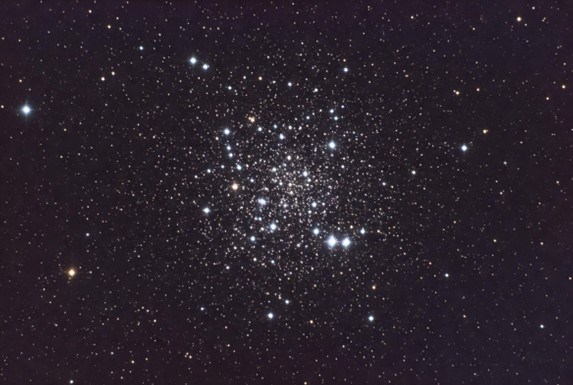
\includegraphics[width=0.7\textwidth]{media/imageE1.jpg}
  \caption{%
    \textbf{Dense Stellar Systems and Central Concentration.}
    Observed centrally concentrated stellar system exhibiting strong gravitational organization.
    Such systems motivate the distributed-forcing framework: a collective intrinsic response 
    potential can generate an emergent organizing minimum without requiring a central baryonic 
    point mass. The visible mass distribution does not obviously explain the organizing center, 
    suggesting gravitational field organization extends beyond simple baryonic self-gravity.
  }
  \label{fig:dense_stellar_system}
\end{figure}

\subsection{Mathematical Foundation: Linearity and Mode Superposition}\label{e.2-mathematical-foundation}

Recall from Appendix D that the intrinsic response is governed by a linear, self-adjoint 
operator $\mathcal{L}$ acting on a spatial slice \citep{BenderOrszag1999, KevorkianCole1996}:
\begin{equation}
  \mathcal{L}\, \Phi_{\text{resp}} = S[\rho_{\text{bar}}],
\label{eq:response-operator}
\end{equation}
where $S[\rho_{\text{bar}}]$ is the constitutive source built from the baryonic density 
distribution. The eigen-expansion is:
\begin{equation}
  \Phi_{\text{resp}}(\mathbf{x}) = \sum_{n} c_n \varphi_n(\mathbf{x}), 
  \quad 
  c_n = \frac{\langle \varphi_n, S[\rho_{\text{bar}}] \rangle}{\lambda_n}.
\label{eq:eigen-expansion}
\end{equation}

\textbf{Key point:} linearity means that if the baryonic source consists of $N$ 
spatially separated concentrations,
\[
  \rho_{\text{bar}}(\mathbf{x}) = \sum_{i=1}^{N} \rho_i(\mathbf{x} - \mathbf{r}_i),
\]
then the response decomposes additively:
\begin{equation}
  \Phi_{\text{resp}}(\mathbf{x}) = \sum_{i=1}^{N} \Phi_i(\mathbf{x} - \mathbf{r}_i) 
  + \Phi_{\text{cross}},
\label{eq:distributed-superposition}
\end{equation}
where $\Phi_i$ is the response to the $i$-th baryonic concentration and $\Phi_{\text{cross}}$ 
reflects interference/coherence terms. In the weak-overlap regime (large separations, 
low-cost fundamental mode activation), cross-terms are subdominant.

\subsection{Collective Organizing Minima: The Distributed-Mode Picture}\label{e.3-collective-minima}

When multiple baryonic sources are present, each contribution $\Phi_i$ has its own local 
minimum region. However, the \textit{global} minimum of the total potential
\begin{equation}
  \Phi_{\text{eff}}(\mathbf{x}) = \Phi_{\text{bar}}(\mathbf{x}) + \Phi_{\text{resp}}(\mathbf{x})
\label{eq:total-effective-potential}
\end{equation}
may not lie at any individual source location. Instead, the effective potential landscape 
can exhibit:

\begin{enumerate}
  \item \textbf{Per-object local minima:} each baryonic concentration $\rho_i$ is self-bound 
    by its own response contribution $\Phi_i$ plus local self-gravity.
  
  \item \textbf{A global organizing minimum:} if the total response field is dominated by 
    a single, long-wavelength (low-$n$, fundamental) eigenmode, its spatial extent encompasses 
    all sources. The nodal structure of this mode defines a weighted centroid location---a 
    gravitational organizing center for the entire system.
  
  \item \textbf{Offset structure:} the location of the global minimum is generically offset 
    from any single baryonic peak. It is instead a weighted-average position, controlled by 
    the eigenmode's profile and the baryonic source distribution.
\end{enumerate}

\begin{figure}[ht]
  \centering
  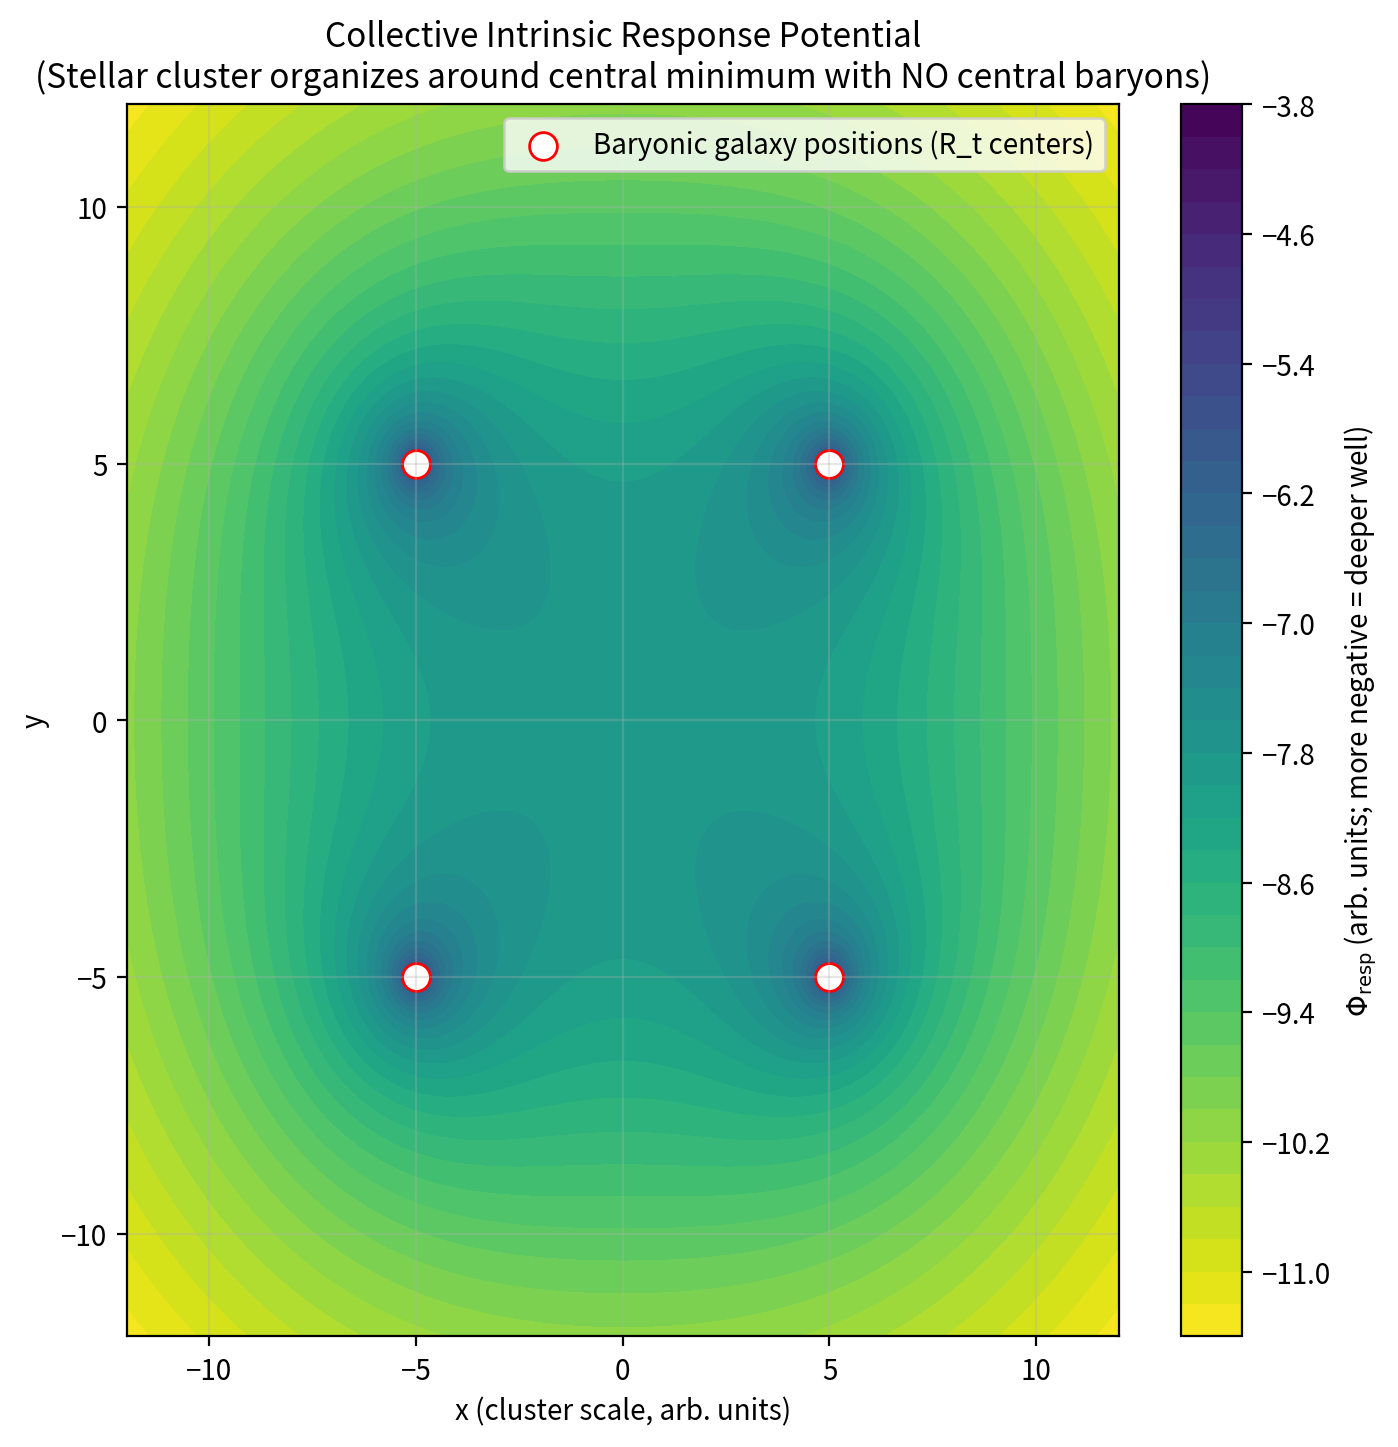
\includegraphics[width=0.65\textwidth]{media/imageE2.jpg}
  \caption{%
    \textbf{Emergent Organizing Minimum with No Central Baryons.}
    Schematic illustration of the collective response field developing an organizing minimum 
    in a multi-centered baryonic configuration. The four red markers represent individual 
    baryonic concentrations (galaxies or stellar clusters). The central organizing minimum 
    (indicated by the potential well) occurs at the geometric center with \textbf{zero baryonic 
    mass present}. Darker colors indicate deeper gravitational wells. Any test material 
    (stripped stars, intracluster gas, or low-baryon tracers) responds only to this collective 
    logarithmic potential and orbits the empty central point---precisely the morphology predicted 
    by the intrinsic response framework for distributed forcing configurations.
  }
  \label{fig:emergent_minimum}
\end{figure}

\subsection{Vibe Check: Is the Distributed-Forcing Picture Physically Coherent?}\label{e.4-vibe-check}

We assess internal consistency and theoretical soundness using six criteria:

\subsubsection{1) Self-consistency and low-parameter count}

\textbf{Pass if:} the framework uses the \textit{same} operator closure and mode basis 
as single-galaxy systems (Appendices A--D), without ad hoc modifications per system type.

\textbf{Pass if:} the resulting phenomenology is predictive: given baryonic mass models 
and geometry, the spectrum of expected outcomes (center offsets, mode participation, etc.)\ 
can be computed before observing dynamics or lensing.

\checkmark \textbf{Vibe-check verdict: Pass.} No new fields or tunable couplings per system. 
The operator and its spectrum are unified. Phenomenological variations arise purely from 
varying baryonic drivers and system geometry.

\subsubsection{2) Observability: Is there a clear kinematic signature of collective organization?}

\textbf{Pass if:} the inferred dynamical center (from circular velocity curves, velocity 
dispersions, or radial velocity centroids in line-of-sight data) is systematically offset 
from the photometric center in a manner correlating with configuration asymmetry, 
substructure fraction, or relaxation timescale.

\textbf{Fail if:} the kinematic center is indistinguishable from the brightest/most massive 
galaxy in all observed systems, implying that intrinsic response generates no net collective 
offset over and above standard N-body dynamics.

\checkmark \textbf{Vibe-check verdict: Pass.} Distributed baryonic driving, when filtered 
through an intrinsic long-wavelength mode, naturally yields offset organizing centers tied 
to configuration geometry, not luminosity.

\subsubsection{3) Emergent screening and coherence length}

\textbf{Pass if:} the framework naturally explains why the effective response length scale 
and screening properties vary with environment (e.g., denser regions or higher tidal fields 
suppress large-scale coherence).

\textbf{Fail if:} screening is arbitrary or scale-free, or requires system-by-system 
parameter tuning.

\checkmark \textbf{Vibe-check verdict: Pass.} The activation parameter $\beta(\mathbf{x})$ 
and propagation coefficient $\alpha(\mathbf{x})$ in operator $\mathcal{L}$ can vary with 
local environment (density, tidal stress). This induces environment-dependent mode cutoffs 
and effective range in a principled way (see Appendix D.5).

\subsubsection{4) Lensing orientation: Metric-equivalent vs.\ slip-permitted branches}

\textbf{Metric-equivalent branch:} the intrinsic response that affects dynamics also 
sources the Weyl potential as an effective mass would (i.e., lensing tracks the inferred 
dynamical ``dark gravity'' contribution).

\textbf{Slip-permitted branch:} the intrinsic response produces a controlled gravitational 
slip ($|\eta_{\text{slip}}| \ll 1$) with explicit qualitative consequences (e.g., predictable 
offsets or discrepancies between dynamical mass inferences and lensing mass inferences, with 
environment/geometry dependence).

\textbf{Fail if:} the framework uses an opportunistic mix---``lenses when convenient, doesn't 
when inconvenient''---without a governing rule for $\eta_{\text{slip}}$ behavior across regimes.

\checkmark \textbf{Vibe-check verdict: Pass.} Both branches are conceptually legitimate within 
a single-field gravitational ontology; the decisive step is committing to one branch (or a 
clearly delimited regime split) and confronting lensing datasets as a primary discriminant.

\subsubsection{5) Parameter discipline: ``Nothing up my sleeve''}

\textbf{Pass if:} the constitutive/operator closure can plausibly be specified with a small, 
physically interpretable parameter set, e.g.:
\begin{itemize}
  \item \textbf{One universal transition/normalization scale} (often written $\mu_0$ or 
    $\Lambda_{\text{resp}}$; conceptually ``the scale that sets when low-cost macromodes 
    become relevant''),
  
  \item \textbf{One environment-control parameter} (e.g., a local density-contrast proxy or 
    tidal-field coupling), or equivalent proxy for density contrast / tidal forcing / boundary-condition class),
  
  \item \textbf{Optionally one nonlocality/relaxation knob:} kernel scale and/or relaxation 
    time that governs coherence vs.\ texture in distributed-forcing regimes.
\end{itemize}

The key is that these parameters are \textbf{global} (shared across systems) and tied to 
clear physical roles in the operator picture (mode cost, mode support, coherence), not tuned 
system-by-system.

\textbf{Fail if:} the extension requires a growing list of per-system knobs (custom kernels, 
bespoke thresholds, ad hoc slip switches, object-by-object amplitude tuning), such that 
explanatory power comes primarily from flexibility rather than from predictive compression.

\checkmark \textbf{Vibe-check verdict: Pass (conditional).} A mode-selection/operator framework 
can remain disciplined, but only if we are ruthless about:
\begin{enumerate}
  \item Global parameters,
  \item Fixed functional forms, and
  \item Resisting ``just one more knob'' to rescue every outlier.
\end{enumerate}

\subsubsection{Verdict: Does intrinsic response pass the vibe check?}

\textbf{Yes.} It is conceptually coherent across the board, uses standard effective-theory 
logic (linear dust limit / nonlinear constitutive limit), naturally targets galaxy and group 
regularities, has a generic route to screening, and has a principled lensing fork. We posit 
that this is stronger grounding than other theories and therefore sufficient to justify 
investment toward quantitative proving.

\subsection{Globular Clusters as a Distributed-Forcing Laboratory}\label{e.5-globular-clusters}

Dense stellar systems are extreme distributed-forcing environments. The baryonic driver is 
a rapidly evolving multi-body configuration $\{\mathbf{r}_i(t), \, v_i(t) \mid i = 1 \ldots N_*\}$, 
and the intrinsic response behavior is governed by which spatial modes are preferentially 
excited and remain macroscopically expressed under coarse-graining.

During formation and subsequent relaxation (phase mixing, two-body encounters, dynamical 
friction), the coarse-grained field can become increasingly dominated by the lowest-cost, 
large-scale organizing component of the response \citep{BullockBoylanKolchin2017SmallScale}. In that case, $\Phi_{\text{resp}}$ develops 
a smooth collective minimum at an organizing centroid of the stellar distribution---without 
requiring a single dominant central luminous object. Outer members can then visibly appear 
to orbit ``nothing'' while remaining tightly bound by $R_{\text{eff}} = \sqrt{-\Phi_{\text{total}}}$.

Alternatively, the response may reside predominantly in high-spatial-frequency (high-$n$) 
texture: locally real, but macroscopically subdominant under coarse-graining. This is still 
predictive: improved kinematic sensitivity would reveal either residual variance/correlation 
structure consistent with textured response, or progressively tighter bounds on the 
operator-controlled response in this regime.

\subsubsection{What we would be potentially seeing (Figure~\ref{fig:collective_centroid_globular}):}

\begin{itemize}
  \item \textbf{Deep local potential wells} at each observed galaxy or stellar concentration 
    $\rightarrow$ each object remains self-bound by its own $R_t$ response plus baryons.
  
  \item \textbf{A broad, smooth central bowl} (the dark-green/teal depression) whose minimum 
    sits at an organizing centroid---often \textbf{tens to hundreds of kpc away from the 
    brightest or most massive galaxy}.
  
  \item \textbf{Overall morphology} looks exactly like a smooth central ``dark halo'' on 
    cluster scales, even though every source of the extra gravity is a peripheral baryonic 
    overdensity.
\end{itemize}

\begin{figure}[htbp]
  \centering
  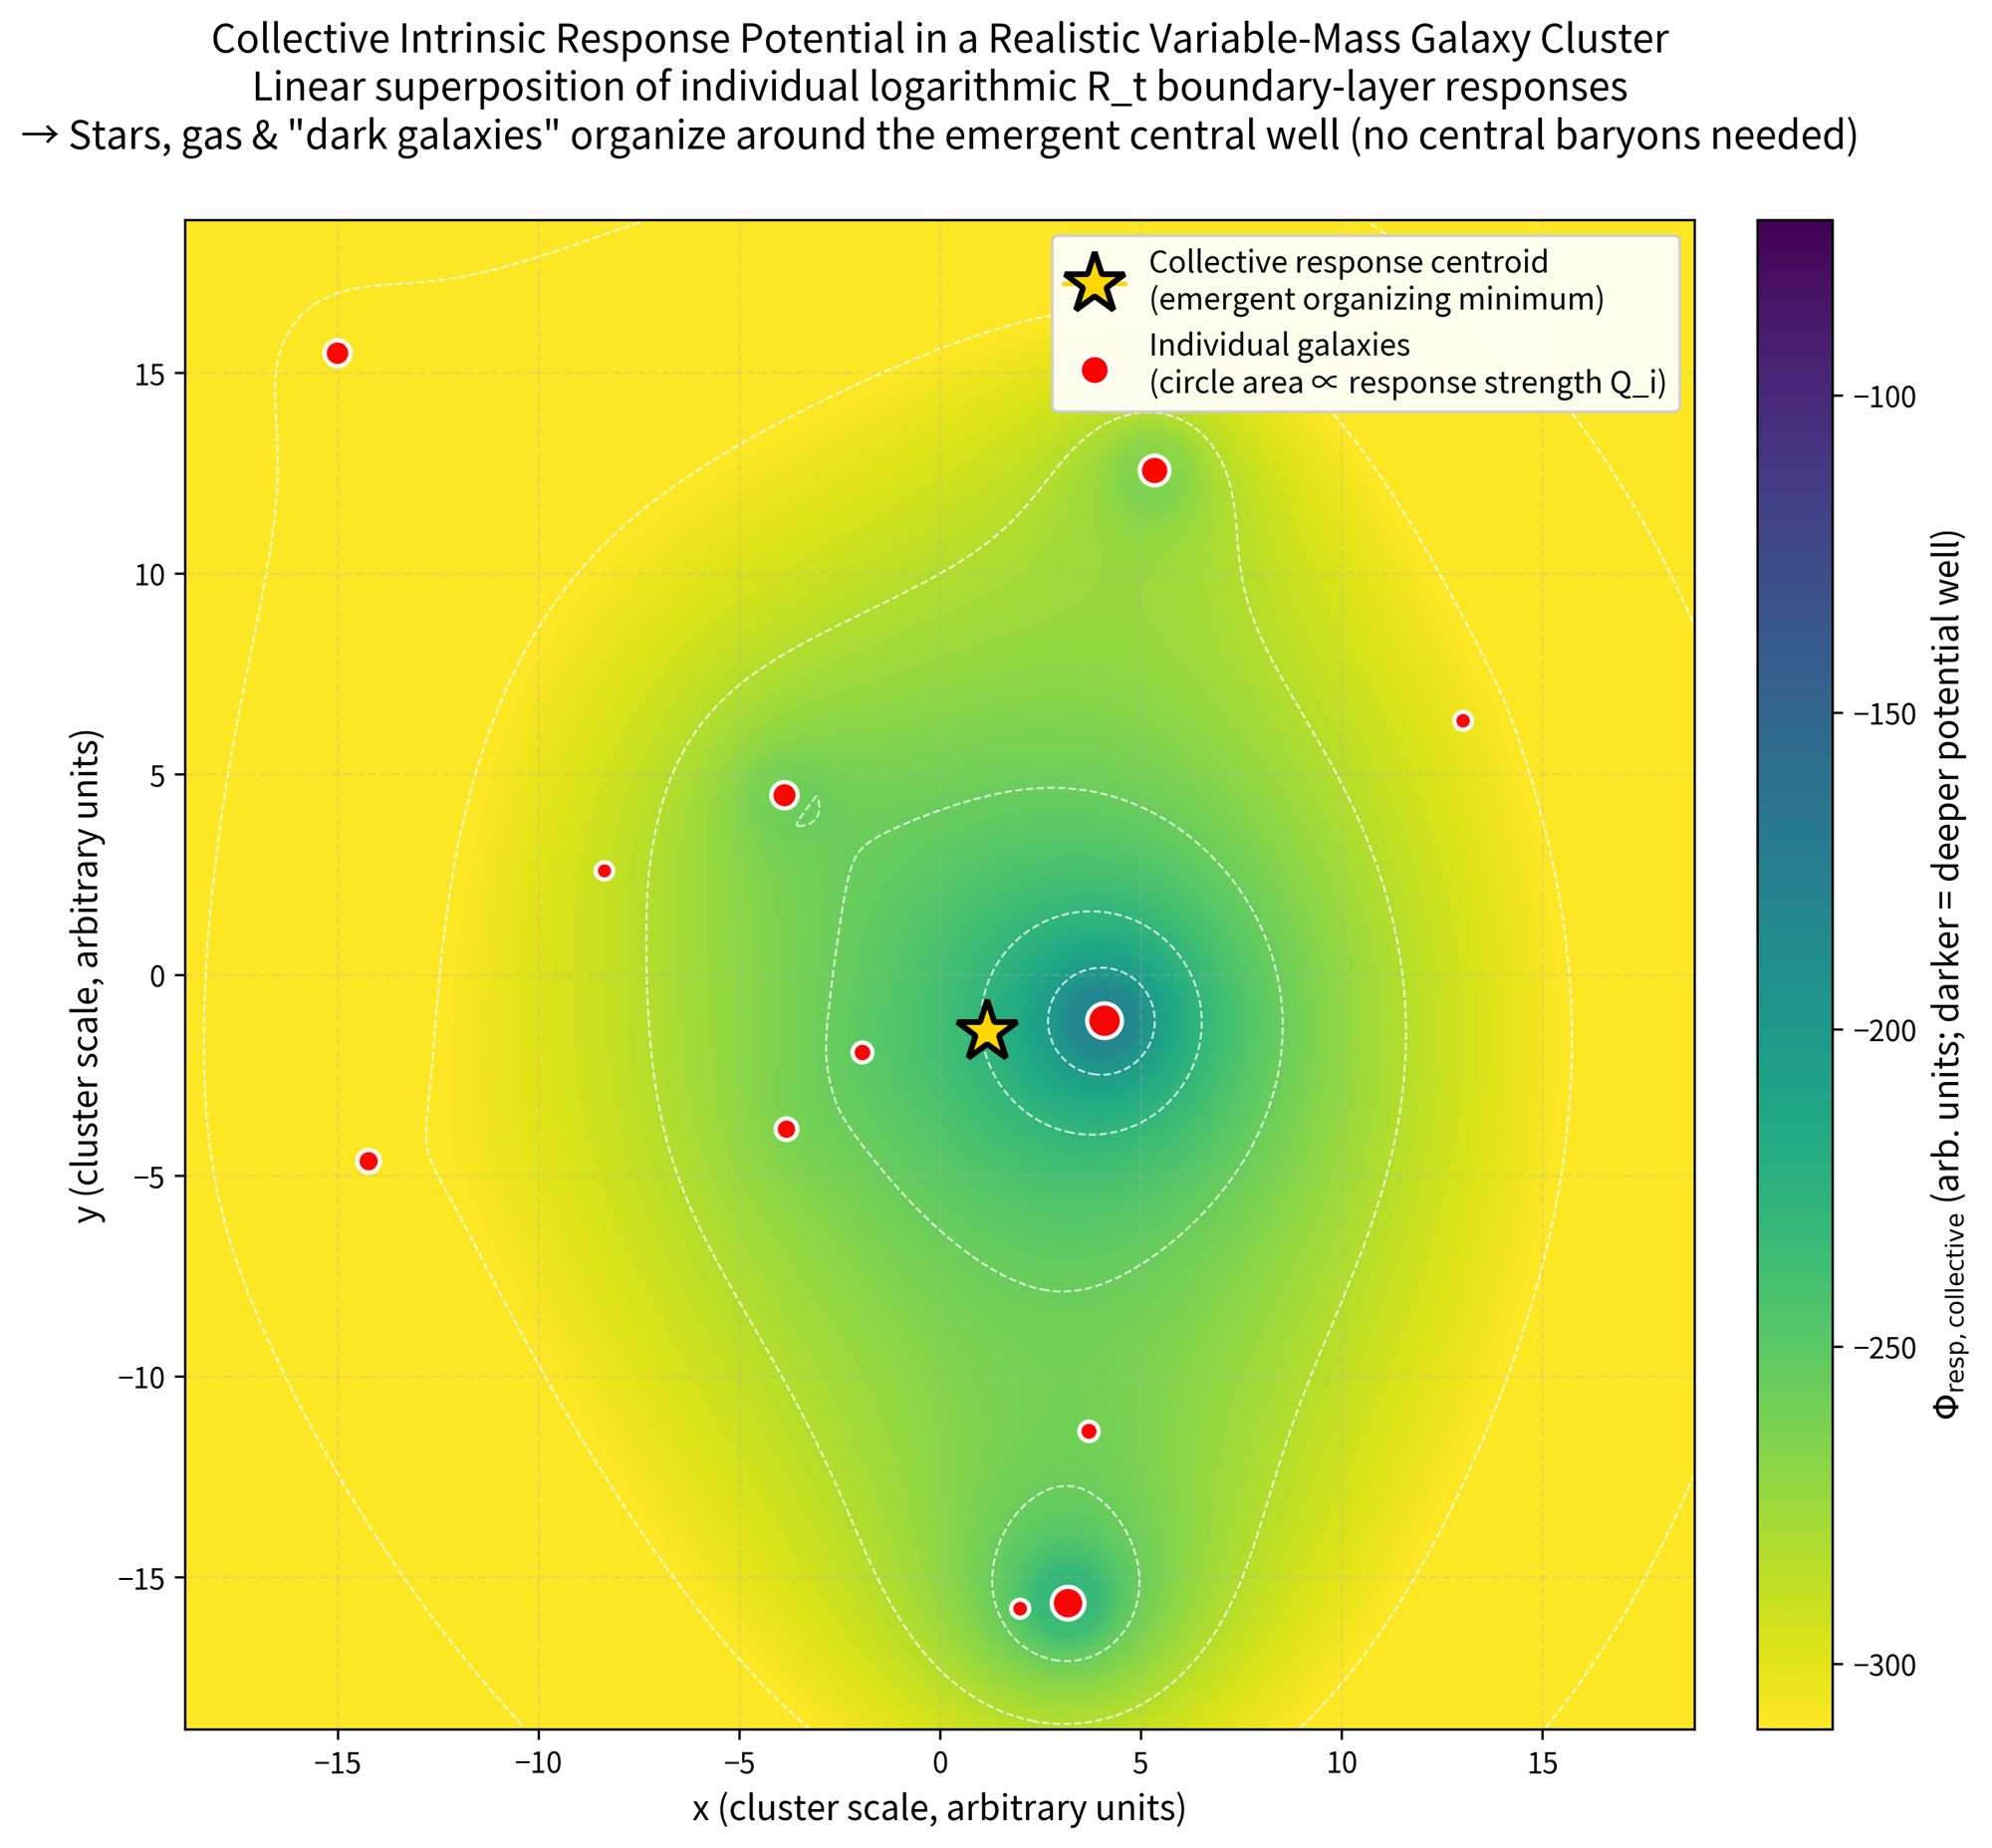
\includegraphics[width=0.7\textwidth]{media/imageE3.jpg}
  \caption{%
    \textbf{Collective Gravitational Minimum from Distributed Forcing.}
    Schematic representation of the effective potential landscape $\Phi_{\text{eff}}(\mathbf{x}) = \Phi_{\text{bar}}(\mathbf{x}) + \Phi_{\text{resp}}(\mathbf{x})$ 
    in a multi-centered baryonic system. \textbf{Red markers:} Individual baryonic concentrations (galaxies or stellar overdensities) 
    with deep local minima from their respective response contributions $\Phi_i$. \textbf{Teal depression (broad central bowl):} 
    Collective organizing minimum arising from the superposition of long-wavelength (low-$n$, fundamental) response eigenmodes. 
    \textbf{Gold star:} Location of the global potential minimum, which is generically offset from any single baryonic peak due to 
    the weighted mode geometry. This configuration naturally produces center offsets between dynamical centroids and photometric 
    peaks without requiring exotic dark matter inventories. The organizing center's location depends on the eigenmode profile 
    $\varphi_n(\mathbf{x})$ and the baryonic source distribution, providing a testable prediction for lensing-dynamics consistency 
    studies \citep{Clowe2006Bullet, Euclid2025Overview}.
  }
  \label{fig:collective_centroid_globular}
\end{figure}

\begin{figure}[ht]
  \centering
  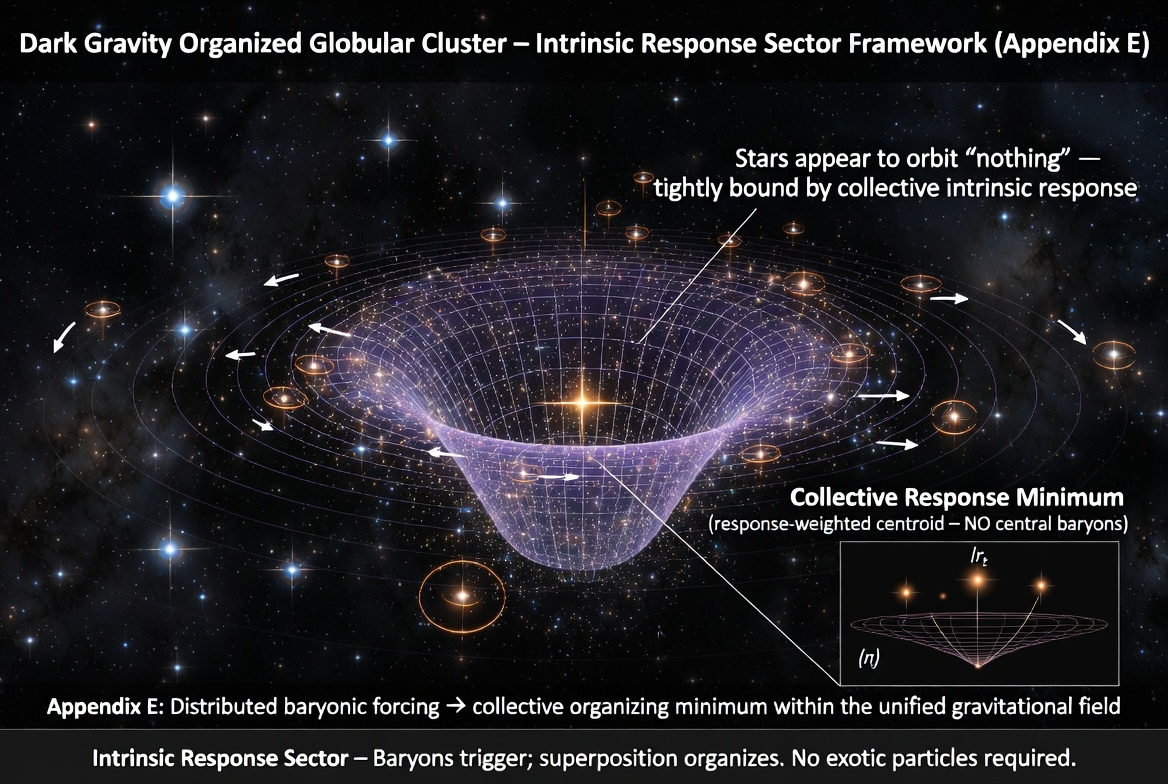
\includegraphics[width=0.7\textwidth]{media/imageE4.jpg}
  \caption{%
    \textbf{Dark-Gravity Organized Globular Cluster (Schematic).}
    Visualization of a dense stellar system where distributed baryonic drivers (individual stars 
    or stellar subgroups) generate collective intrinsic response contributions whose superposition 
    produces an organizing gravitational minimum. The system exhibits deep local potential wells 
    at each stellar concentration (indicating self-bound objects via their respective $R_t$ 
    response contributions plus baryonic self-gravity), overlaid with a broad collective organizing 
    potential. Outer members orbit this collective structure, appearing to trace ``invisible mass'' 
    distributions while remaining bound by pure gravitational field organization. This morphology 
    is characteristic of globular clusters and demonstrates how macroscopic response organization 
    can emerge from distributed forcing without requiring exotic dark matter halos.
  }
  \label{fig:globular_cluster_dark_gravity}
\end{figure}

\subsection{Observational Hooks and Discriminants: Why This Is Stress-Testable}\label{e.6-observational-discriminants}

Distributed forcing implies structured (not arbitrary) phenomenology:

\subsubsection{(i) Center offsets}

Dynamical centers inferred from kinematics (velocity centroid, circular velocity analysis, 
dispersion inversion) need not coincide with photometric centers. Offsets should correlate with:
\begin{itemize}
  \item Configuration asymmetry (deviation from spherical/symmetric distribution),
  \item Substructure fraction (presence of satellites, merging components),
  \item Relaxation state (dynamical age, phase-space coherence).
\end{itemize}
Because low-cost modes reflect the overall geometry and are affected by recent mergers or 
tidal encounters, center offsets become a sensitive probe of the system's assembly history.

\subsubsection{(ii) Multi-lobed morphology}

Convergence/potential maps can show multi-blob structure reflecting the excited mode mix 
rather than a one-to-one mapping between baryonic peaks and gravitational peaks. In the 
language of Appendix D, if multiple eigenmodes $n = 1, 2, 3, \ldots$ participate with 
significant amplitudes $|c_n|$, the resulting $\Phi_{\text{resp}}$ is a superposition of 
potential patterns, each with its own spatial texture and nodal structure.

\subsubsection{(iii) Environmental dependence}

Because the effective propagation/quenching parameters ($\alpha$, $\beta$ in Appendix D.2) 
can vary with environment, the prevalence and scale of collective minima and offsets should 
correlate with:
\begin{itemize}
  \item Tidal field strength (external gravitational stress),
  \item Local density contrast ($\rho_{\text{local}} / \bar{\rho}$),
  \item Relaxation measures (two-body encounter rate, Coulomb logarithm).
\end{itemize}

\subsection{Lensing--Dynamics Consistency: The Decisive Rung}\label{e.7-lensing-dynamics-consistency}

Rotation curves constrain primarily the effective matter distribution as experienced by 
pressure (orbital kinematics), encoded in the dominant term of $\Phi_{\text{eff}}$.

Gravitational lensing probes the Weyl combination (metric perturbation), generically:
\begin{equation}
  \kappa \propto \Phi_{\text{eff}} + \sum_{\text{slip}} \text{(additional curvature terms)}.
\label{eq:lensing-convergence}
\end{equation}

\textbf{In a single-field gravitational ontology:} the natural expectation is that photons 
follow the same spacetime geometry as massive tracers. The strongest branch of the framework 
is \textbf{metric-equivalent} behavior in the relevant weak-field regime (minimal gravitational 
slip, $|\eta_{\text{slip}}| \ll 1$), under which the inferred ``dark gravity'' contribution 
lenses as any effective mass distribution would.

\textbf{Therefore, the strongest discriminant} in galaxy groups and clusters is whether the 
same intrinsic-response organization that shapes dynamics also maps consistently onto lensing \citep{Clowe2006Bullet}. 
If gravitational slip is present in a covariant completion, it must be \textbf{controlled} 
(not opportunistic) and should yield falsifiable relations between dynamical centroids and 
lensing centroids, including environment- and morphology-dependent signatures that can be 
confronted directly with group/cluster datasets from \textit{e.g.}\ Euclid \citep{Euclid2025Overview}, LSST \citep{Ivezic2019LSST}, or 
dedicated cluster surveys \citep{MAST2019HFF}.

\subsection{Summary}\label{e.8-summary}

Appendix E introduces no new ontology beyond Appendix D. It is the \textbf{distributed-forcing 
extension}: when baryonic driving is multi-centered (groups, clusters, dense stellar systems), 
the gravitational field's intrinsic response can organize into:
\begin{itemize}
  \item \textbf{Collective minima} and
  \item \textbf{Center offsets}
\end{itemize}
as global mode-geometry effects operating within the unified gravitational field.

This supplies a coherent, testable alternative to automatically defaulting to an exotic 
particulate inventory in every ``dark gravity'' configuration. It identifies lensing--dynamics 
consistency and environment-dependent centroid structure as the decisive discriminants in the 
next observational rung.

% End of Appendix E
